\documentclass[acmtog, authorversion]{acmart}
\usepackage[htt]{hyphenat}
\usepackage{graphicx}
\usepackage{lipsum}
\usepackage{pgfgantt}
\usepackage{enumitem}
\usepackage{booktabs}

\newlist{questions}{enumerate}{2}
\setlist[questions,1]{label=\textbf{RQ\arabic*.},ref=RQ\arabic*}
\setlist[questions,2]{label=(\alph*),ref=\thequestionsi(\alph*)}
\graphicspath{{images/}}

\AtBeginDocument{%
  \providecommand\BibTeX{{%
    \normalfont B\kern-0.5em{\scshape i\kern-0.25em b}\kern-0.8em\TeX}}}

\setcopyright{acmcopyright}
\copyrightyear{2023}
\acmYear{2023}

\acmConference[TScIT 39]{39$^{th}$ Twente Student Conference on IT}{July 8,
  2023}{Enschede, The Netherlands}

\begin{document}

\title{Satellite to Radar: Sequence to Sequence Learning for precipitation nowcasting}

\author{Mark Bruderer}
\email{m.a.bruderervanblerk@student.utwente.nl}
\affiliation{%
  \institution{University of Twente}
  \streetaddress{P.O. Box 217}
  \city{Enschede}
  \country{The Netherlands}
  \postcode{7500AE}
}

\renewcommand{\shortauthors}{Mark Bruderer}

\begin{abstract}
\section*{Abstract}
The forecasting of rain is a complex problem with centuries of scientific work. The implications of weather for individuals and companies continue to be important. Machine Learning approaches have been shown to outperform state of the art physics based models of weather for short term predictions. We introduce a new type of model \textbf{Sat2Rad}. Our model takes as input multi-spectral satellite data and outputs radar reflectivity at a set of time-steps ranging from 15 to 180 minutes in the future.
\end{abstract}

\keywords{Machine Learning, Sequence to Sequence, Radar, Satellite, Storms, Forecasting}

\settopmatter{printacmref=false}

\begin{teaserfigure}
  \includegraphics*[width=\textwidth, trim= 0in 0.0in 0in 16.0in]{images/lightning.jpg}
  \caption{A supercell thunderstorm at twilight in SW Oklahoma.^1}
  \Description{A supercell thunderstorm at twilight in SW Oklahoma.}
  \label{fig:teaser}
\end{teaserfigure}

\maketitle

\section{Introduction} \label{introduction}

Precipitation forecasting is essential to reduce the risk of life threatening situations. Different types of rainfall ranging from mist to heavy rain have a major impact for different societal sectors including agriculture, aviation, outdoor events, and the energy industry.
By having timely and accurate predictions of rainfall which in turn indicate the potential for destructive storms we can prevent injuries, assist companies in predicting energy production and use resources efficiently.
\medskip

% Predicting and understanding weather has become crucial in a number of industries, including agriculture, autonomous driving, aviation, or the energy sector. For example, weather conditions play a significant role for aviation and logistics companies in planning the fastest and safest route. Similarly, renewable energy companies need to be able to predict the amount of energy they will produce at a given day. As a consequence various weather models have been developed and are being applied all over the world. Unfortunately, these models often require highly specific information about the atmosphere and exact conditions.

% explain what storms are:
% - why are storms important
% - what are storms => how they from
A particularly strong threat is posed by rain storms and thunderstorms. Storms are one of the most destructive weather events in nature, capable of destroying human structures and even lead to loss of life \cite{noaa-national-severe-storms-laboratory-no-date}. Predicting storms is crucial and presents it's own set of challenges.
\medskip

% explain how to currently predict storms
At present meteorologists are able to successfully predict many instances of precipitation. Techniques that are used in practice range from manual analysis of current weather data (e.g radar or satellite images) to complex physics based simulations of our atmosphere with Numerical Weather Prediction (\textsc{NWP}) models.
\textsc{NWP} models predict precipitation based on \textit{optical flow}. Optical flow functions in two steps, first cumulonimbus clouds are identified, and then their movement is tracked to predict the location of precipitation. Thus in the case of \textsc{NWP} models, the \textit{cell-lifecycle} \cite{noaas-national-weather-service-no-date} is not taken into account \cite{prudden2020review}.
\medskip

% explain machine learning approaches
Machine Learning (\textsc{ML}) approaches have also been developed to predict precipitation. An improvement of machine learning models over \textsc{NWP} models is that they are much faster to produce predictions, thus ML models are more suitable for real-time or near-real-time predictions, such as required in disaster response and energy management. According to the universal approximation theorem \cite{cybenko-1989}, deep neural networks have the property of being able to approximate any function provided they have the correct weights, thus it is suggested that machine learning models can incorporate sources of predictability beyond optical flow such as the cell-lifecycle among others \cite{prudden2020review}.
\medskip

% explain our approach
Thus far most machine learning approaches for precipitation nowcasting have focused on predicting a next frame in a time series of radar reflectivity data \cite{shi2017deep, convlstm, rainet}. However taking this approach may eliminate the possibility of learning the cell-lifecycle, due to the fact that the model only sees precipitation itself but not the cloud that is causing the precipitation.
\medskip

% "Yet the key issue of precipitation prediction – the anticipation of convective initialization, as well as the growth and dissipation of precipitation in the imminent future – still appears to be unresolved" 

We propose to use multi-spectral satellite data to learn spatio-temporal mappings between sequences of satellite data and precipitation data. If this is successful \textit{cumulonimbus} clouds could be predicted from when they are mere \textit{cumulus} clouds and prior. An additional advantage is that satellite data as opposed to radar data is readily available over oceans and remote communities which allows for the prediction of precipitation over these regions. We will work towards creating a model by answering the following main research question:
\smallskip

% Most physical models are based on the extrapolation of the detected Cbs with atmospheric motion vectors (AMV; see [14] and the references therein). This approach works well as long as the cells do not decay during the prediction period. Unfortunately, cells usually do decay after a certain lifetime, such that this effect occurs regularly. Further, newly developed cells cannot be captured by extrapolation of detected cells. These are serious drawbacks of the AMV approach. The quite good results achieved with deep learning indicate that the training process might enable the network to gain information on the life cycles of cells (decay, newly developed cells). The network seems to be able to learn to a certain extent whether Cbs decay or newly develop within the prediction period or not, and we believe this is crucial for lead times around or larger than 180 min, as the lifetime of regular Cbs is usually shorter than this; see, e.g., 
% - 

% Radar has been the primary tool for predicting precipitation for decades, but it has limitations, such as its limited range and the fact that it cannot penetrate through heavy precipitation. This makes it difficult to predict precipitation in areas that are far from the radar, such as remote regions and over the ocean.

% Satellite data, on the other hand, can provide a global view of weather patterns and can be used to fill in gaps in radar coverage. Satellites can also provide information about cloud temperature, humidity, and other atmospheric conditions that can be used to infer the presence of precipitation. Additionally, satellite data can be useful for predicting the onset and duration of precipitation events, which can be valuable information for planning and emergency response.

% However, using satellite data for precipitation nowcasting also presents some challenges, such as the need to develop accurate algorithms for translating satellite data into precipitation estimates. These algorithms must take into account factors such as the altitude of the clouds, the types of precipitation (e.g. rain, snow, or hail), and the intensity of the precipitation. Despite these challenges, the use of satellite data for precipitation nowcasting shows great promise and has the potential to improve our ability to predict precipitation in a variety of settings.

\textbf{RQ1}: \textit{How can a deep learning model be trained to predict radar data with multi-spectral satellite data ?}
\smallskip

This research question will be answered by looking at the following sub research questions:
\begin{enumerate}
    \item \textit{what is necessary to build a well performing model ?}
    \item \textit{what methods can be used to create this model ?}
    \item \textit{what is the effectiveness of the trained model ?}
    \item \textit{what are the conditions under which the model can and cannot be used ?}
\end{enumerate}

\section{Main Contribution}
This proposal has the potential to contribute a deep learning model capable of predicting precipitation in the short term with only satellite images.

\section{Related Works}

In this section we will discuss the existing work in precipitation nowcasting via machine learning. This section is structured by the type of input data used in the approaches, first we list radar based learning and then we discuss satellite based approaches.

\subsection{Radar Based Nowcasting}

Recurrent neural networks (\textsc{RNNs}) have been created to learn temporal relationships in data, therefore they are a natural candidate to the task of learning spatio-temporal patterns of weather. The \textsc{LSTM} architecture was developed by Hochreiter and Schmidhuber \cite{lstm}, to solve the problem of vanishing and exploding gradients in RNNs and is widely used. Taking LSTM as a base and adapting the weights to kernels, \textsc{ConvLSTM} \cite{convlstm} was introduced for the task of precipitation nowcasting. Multiple layers of ConvLSTM are used in this paper to obtain a sequence to sequence architecture. A further improvement of ConvLSTM is \textsc{trajGRU} which was proposed by Shi et al. \cite{shi2017deep} to be able to learn the \textit{location-variant} structure for recurrent connections.
\medskip

Pure convolutional neural networks have also been used to predict precipitation. As demonstrated by Bai et al. and Gering et al. \cite{bai2018empirical, gehring2017convolutional} convolutional neural architectures can outperform recurrent neural networks for a variety of sequence modelling tasks. This is the reason why many works on precipitation nowcasting have opted for pure convolutional networks \cite{rainet,agrawal2019machine}.
\medskip

Due to machine learning models attempting to minimize loss, \textit{blurry predictions} can be produced by models. This can be alleviated by using generative models which sample from the possible futures and do not seek to provide a best average fit. Generative Adversarial Networks have been successfully applied to the task of precipitation nowcasting \cite{Ravuri_2021}.

\subsection{Satellite Based Nowcasting}

In their study Chen et al. built a \cite{precipitationEstimationFromSat} MLP to forecast radar data from satellite data. The researchers used a combination of low earth orbit satellite passive microwave and infrared channels from two different satellites. Their model is developed to predict up to 1.5 hours in the future by recursive predictions of the model.
\medskip

A study that does not predict precipitation but uses lightning as a marker for extreme precipitation was performed by Brodehl et al. \cite{predictionLightning} this study uses a convolutional network to predict lightning events, and contributes the important observation that both the visual and infrared channels are significant in differing ways to predict lightning.
\medskip

The approach taken by the researchers of MetNet \cite{sønderby2020metnet} is to combine a convolutional block for spatial downsampling, then a ConvLSTM block for temporal encoding and finally a Axial attention block \cite{vaswani2017attention}. MetNet is able to perform more accurate forcasts than NWP models for up to 8 hours. In this study the input data that is used is both satellite and radar data as well as the elevation, time of the year and latitude and longitude values.

\section{Background}
In order to understand this research it is important to be acquainted with the machine learning techniques that will be used. Furthermore insight into this study can be enhanced by having more in depth information on the used data-sets and the meteorological theory.
\medskip

For the machine learning aspect of this research it is important to understand multi layer perceptrons (\textsc{MLPs}) \cite{schmidhuber2022annotated}. Furthermore it is important to understand convoutional neural networks and what benefits they afford in relation to \textsc{MLPs} \cite{oshea2015introduction}. It is also crucial to have an understanding of recurrent neural networks (RNNs) and their extension to include convolutions \cite{convlstm}.
\medskip

To have an understanding of the meterological context of this project it is recommended to have an understanding of radar data \cite{rinehart1991radar}, satellite data specifically the kind used in this project \cite{schmid-no-date}.

\section{Methods}

% Can also be a new way to solve the problem or a hybrid method (mixed strategy, etc..). In this case, it would be nice to see a description of the steps which are followed in order to solve the problem.

In this section we will discuss how we will approach the answering of our research questions.
\medskip

In our first and second sub-research questions we will perform a more comprehensive literature review to elicit the necessary methods that are required to create and evaluate the  model for example: suitable loss functions from superzoom studies, metrics which are suitable for meterological applications and methods to perform evalutations. These insights will be necessary to the work in sub-research questions 3 and 4.
\medskip

To answer our third sub-research question, we foresee to create a baseline model with a Convolutional LSTM architecture, if this succeeds we will expand this network by adding convolutions for spatial downsampling and axial attention in order to improve the accuracy of our model as done in \cite{sønderby2020metnet}.
\medskip

To answer the final sub-research question, we will evaluate the model to identify the suitability of our trained model in different meteorological situations.

\section{Expected Results}

\subsection{Data}

\subsubsection{Dataset Details}

We have obtained a multi-year structured archive of radar composites with a temporal resolution of 5 minutes. These radar composites are made from 5 Doppler radars that provide a good coverage of the Benelux area (See figure \ref{fig:source}). The readings of these radars can be combined to produce radar reflectivity data (see figure \ref{fig:reflect}).
\medskip

Additionally we have obtained satellite data from \textsc{EUMETSAT} at a \texttt{3x3km} spatial resolution and 15 minute temporal resolution. This data has been captured with the \textsc{SEVIRI} sensor \cite{schmid-no-date}, which produces multi-spectral satellite imagery (See figures \ref{fig:vis} and \ref{fig:infra}).

\begin{figure}[]
    \centering
    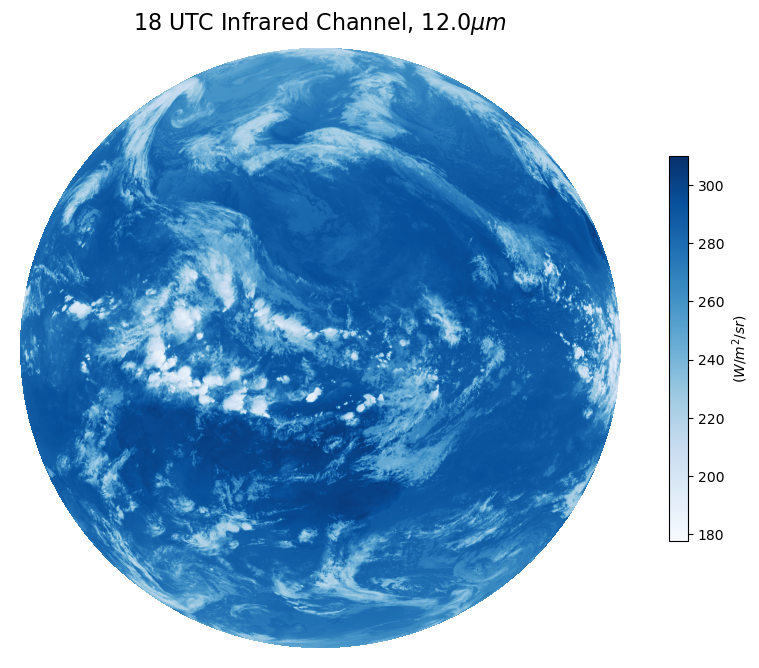
\includegraphics[width=225]{report/images/infrared.png}
    \caption{Satellite Image: Infrared Channel 18UTC 12.0\mu m}
    \label{fig:infra}
\end{figure}

\subsubsection{Data Cleaning} \textit{UMAP} \cite{mcinnes2020umap} will be used to cluster the data from the satellite and radar to find outliers and potential data imbalances.

\subsubsection{Preprocessing Details} Several options exist for preprocessing of the data. One could reproject the satellite images to match the area and geographic projection of the radar images, however this requires heavy computation and studies such as \cite{sønderby2020metnet} have shown the importance of the context (i.e data from outside the region of interest) for the predictions, therefore we will first experiment with leaving the data in the current projection. We will standardize the pixel data to floating point data between \texttt{0} and \textt{1}.

\subsection{Implementation Details}

We plan to work with \texttt{pytorch} due to the higher degree of availability of open-source model implementations that we can use as a base for our work, for instance this repository: \cite{openclimatefix-no-date}.

\subsection{Metrics}
We plan to use the following metrics to evaluate our model:

\begin{equation}
MSE = \frac{\sum (\hat{y_i} -y_i)^2}{n}
\end{equation}

\begin{equation}
MAE = \frac{\sum |\hat{y_i} -y_i|}{n}
\end{equation}

\begin{equation}
RMSE = \sqrt{\frac{\sum (\hat{y_i} -y_i)^2}{n}}
\end{equation}

Additional metrics come from the study \cite{shi2017deep}, where the authors created \textit{B-MSE} and \textit{B-MAE} due to the fact that the frequencies of different rainfall levels are imbalanced. Models trained with conventional \textit{MSE} or \textit{MAE} are biased towards predicting low amounts of precipitation. This can be solved with a loss function that weights the higher precipitation more strongly. The weighting function \textit{w} can be found in the study as well.

\begin{equation}
BMSE = \frac{\sum w(\hat{y_i}) \cdot (\hat{y_i} -y_i)^2}{n}
\end{equation}

\begin{equation}
BMAE = \frac{\sum w(\hat{y_i})  \cdot (\hat{y_i} -y_i)^2}{n}
\end{equation}

\subsection{Experiments}

The input and output data will be the full data as discussed in the data section, and will not change based on the experiments, since we know from literature that all the data from satellite channels can be useful.

\begin{enumerate}
    \item Use ConvLSTM architecture.
    \item Use MetNet architecture
    \item Evaluate the best performing model by running it over a month of data, and analyse the performance by performing aggregations of the predicted data and the ground truth.
\end{enumerate}

\section{Time Planning}
In this section we discuss our planning for the execution of the study in this proposal. In the \textit{gantt} chart you can see that we begin by getting a go for the proposal. Then we start by answering sub-research question 1 and 2 then we proceed by answering sub-research question 3 and finally we bring the research to a close with sub-research question 4.

\medskip

\begin{ganttchart}[hgrid,vgrid,
bar/.append style={fill=blue!50},
group/.append style={draw=black, fill=gray!50},
milestone/.append style={fill=yellow!50, rounded corners=3pt}]{1}{11}
  \gantttitle{\textbf{Planning Table}}{11} \\
  \gantttitlelist{1,...,11}{1} \\
  \ganttgroup{Research}{1}{11} \\
  \ganttbar{Proposal}{1}{2} \\
  \ganttmilestone{Draft Proposal}{2} \\
  \ganttmilestone{Final Proposal}{3} \\
  \ganttbar{Writing}{3}{10} \\
  \ganttmilestone{Draft Paper}{9} \\
  \ganttmilestone{Final Paper}{10} \\
  \ganttbar{Presentation}{11}{11} \\
  \ganttbar{subRQ1-2}{3}{3} \\
  \ganttbar{subRQ3}{4}{8} \\
  \ganttbar{subRQ4}{8}{9} \\
  \ganttlink{elem8}{elem9}
  \ganttlink{elem9}{elem10}
  \ganttlink{elem1}{elem4}
\end{ganttchart}


\section{Conclusions}
At this point in the research we have created an \hyperref[introduction]{introduction for the research}. We have also performed a literature review of available work in the field of precipitation nowcasting. We have written the methods that we will use to perform the research and listed expected results. And we have visualized some of the data from our dataset.

% \begin{acks}
% I would like to thank my supervisor from the university of twente Elena Mocanu, for her help in writing the paper. Furthermore I would like to thank I would like to thank Dina Lazorkeno for proofreading my thesis.
% \end{acks}

\bibliographystyle{ACM-Reference-Format}
\bibliography{ref}

\newpage
\appendix
%Appendix A
\section{Appendix}

\begin{figure}
    \centering
    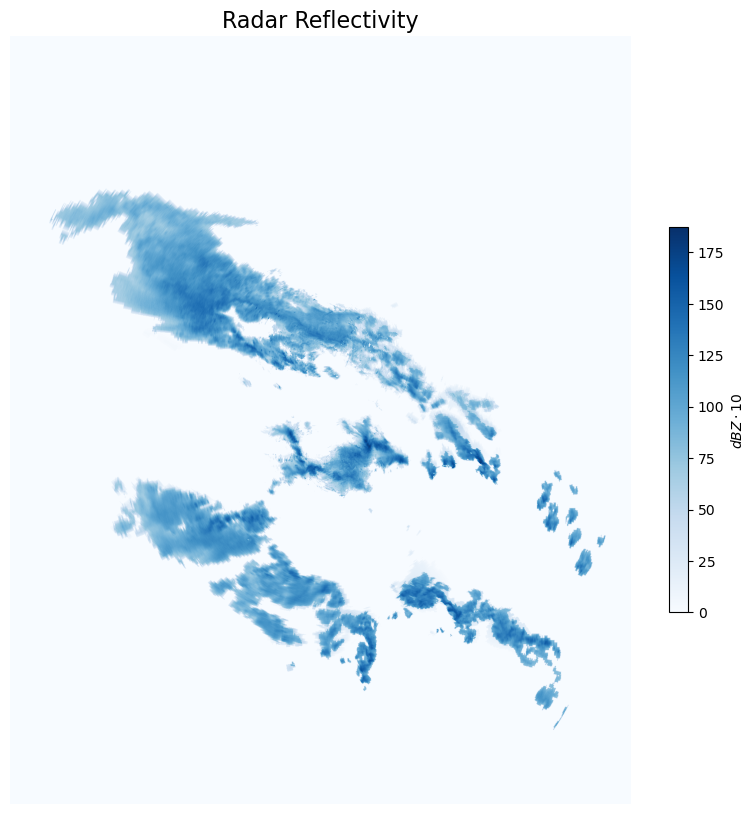
\includegraphics[width=225]{report/images/radar_reflectivity.png}
    \caption{Radar Reflectivity}
    \label{fig:reflect}
\end{figure}

\begin{figure}
    \centering
    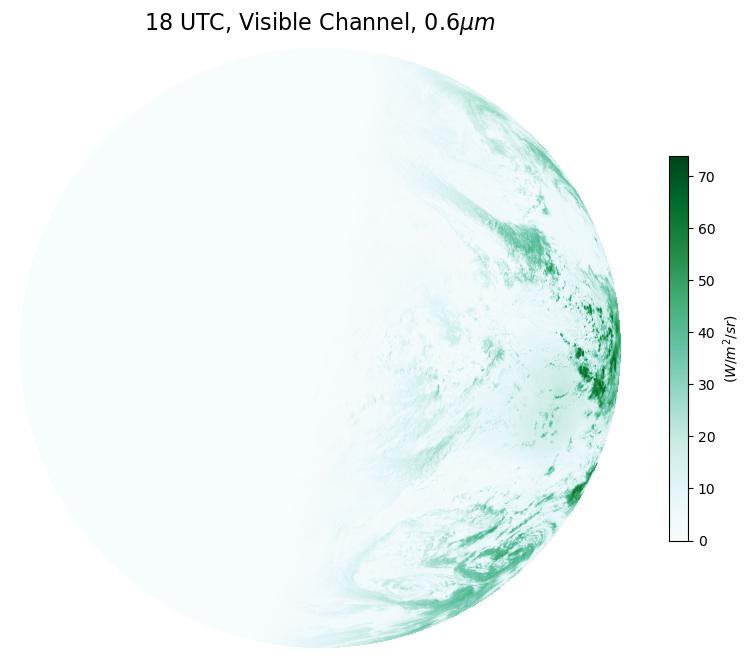
\includegraphics[width=225]{report/images/vis_006.png}
    \caption{Satellite Image: Visible Channel 18UTC 0.6\mu m}
    \label{fig:vis}
\end{figure}

\begin{figure}
    \centering
    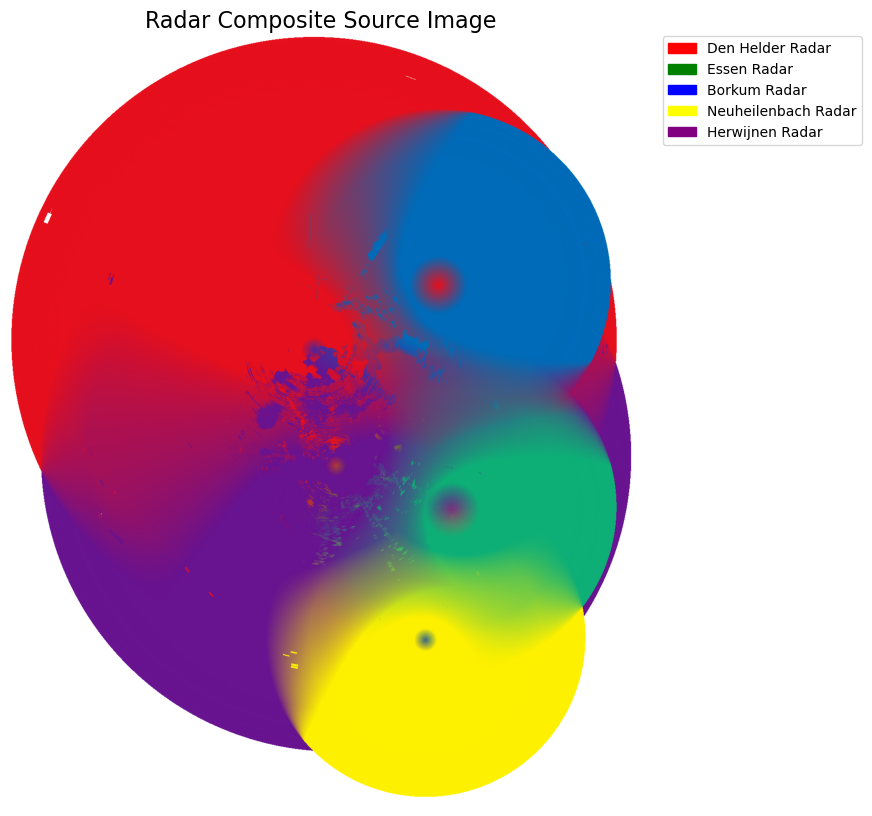
\includegraphics[width=225]{report/images/radar_source.png}
    \caption{Satellite Image: Infrared Channel 18UTC 12.0\mu m}
    \label{fig:source}
\end{figure}


\begin{table}[h]
\caption{Reflectivity in dBZ versus Rainrate}
\begin{tabular}{@{}llll@{}}
\toprule
LZ(dBZ) & R(mm/h) & R(in/h)        & Intensity             \\ \midrule
5       & (mm/h)  & \textless 0.01 & Hardly noticeable     \\
10      & 0.15    & \textless 0.01 & Light mist            \\
15      & 0.3     & 0.01           & Mist                  \\
20      & 0.6     & 0.02           & Very light            \\
25      & 1.3     & 0.05           & Light                 \\
30      & 2.7     & 0.10           & Light to moderate     \\
35      & 5.6     & 0.22           & Moderate rain         \\
40      & 11.53   & 0.45           & Moderate rain         \\
45      & 23.7    & 0.92           & Moderate to heavy     \\
50      & 48.6    & 1.90           & Heavy                 \\
55      & 100     & 4              & Very heavy/small hail \\
60      & 205     & 8              & Extreme/moderate hail \\
65      & 421     & 16.6           & Extreme/large hail    \\ \bottomrule
\end{tabular}
\end{table}



\end{document}
